%chap 4
\chapter{مدل پیشنهادی}
\thispagestyle{empty}
\section{مقدمه}
در این بخش روش پیشنهادی در این پایان‌‌نامه که یک مدل بر پایه‌ی شبکه‌های عصبی برای تشخیص همزمان احساس و موضوع از داده‌های متنی است ارائه می‌‌گردد. همانطور که پیش از این نیز ذکر شد مدل پیشنهادی در این پایان‌‌نامه گسترش یافته و تلفیقی از چند مدل شناخته شده در زمینه‌ی مدل‌سازی احساس و موضوع و همچنین تشخیص توزیع‌های احتمالی‌ موجود در داده‌های ورودی است، لذا در بخش‌های پیش‌ر‌‌و ضمن معرفی‌ کامل این مدل‌ها و تعریف ساختار و 
نحو‌ه‌ی عملکرد هرکدام به مدل پیشنهادی در این پایان‌‌نامه می‌‌رسیم و آن را به طور کامل مورد بررسی‌ قرار داده و تعریف می‌‌کنیم.

\section{مدل پایه}
\label{chap4sec2}
مدل پایه در این پایان‌‌نامه  شبکه عصبی ماشین بلتزمن محدود است که پیش از این در بخش
\ref{chap3sec2sub1}
 آن را
RBM
نامیدیم و به صورت مختصر معرفی‌ گردید.
RBM
که در شکل
\ref{chap4-fig1}
نشان داده شده است،
 RBM 
 یک مدل بدون نظارت برای داده‌های باینری است که در دسته‌ی مدل‌های مولد احتمالاتی  قرار می‌گیرد. در این مدل با بیشینه کردن یک تابع انرژی، یا کمینه کردن مقدار منفی‌ آن که به صورت رابطه‌ی
\begin{align}
	\centering
	\label{chap4-eq1}
	E(\textbf{v},\textbf{h}) = -\sum_{i} \sum_{j} v_iW_{ij}h_j - \sum_i v_ia_i - \sum_j h_jb_j
\end{align}
تعریف می‌‌شود، توزیع‌های احتمالی‌ موجود در داده‌های ورودی یاد گرفته می‌شود و از داده‌های ورودی ویژگی‌ استخراج می‌‌گردد. در رابطه‌ی
\ref{chap4-eq1}
مجموعه‌ی پارامترهای مدل به صورت
$\theta = \{W, \textbf{a}, \textbf{b}\}$
است.
$W_{D \times H}$
ماتریس وزن بین لایه‌ی ورودی و لایه‌ی پنهان است، که در آن
$D$
اندازه بردار ورودی و
$H$
اندازه لایه‌ی پنهان هستند.
$\textbf{a}$
بردار بایاس لایه‌ی ورودی با اندازه
$D$
و
$\textbf{b}$
بردار بایاس لایه‌ی پنهان با اندازه
$H$
 است. همان‌طور که در بخش 
 \ref{chap3sec2sub1}
نیز بیان گردید در مدل
 RBM
 داده‌های ورودی و لایه‌ی پنهان متناظر با آن که توسط مدل از بردار ورودی بدست می‌‌آید هر دو در حالت باینری (۰ یا ۱) هستند که این امر یکی‌ از محدودیت‌های این روش است.


در مدل
RBM
احتمال هر ترکیب
$(\textbf{v},\textbf{h})$
از رابطه‌ی
\begin{align}
	\centering
	\label{chap4-eq2}
	p(\textbf{v},\textbf{h}) = \dfrac{1}{Z(\theta)} e^{-E(\textbf{v},\textbf{h})}
\end{align}
بدست می‌‌آید که در آن
$Z(\theta)$
تابع قسمت‌بندی است که مقدار آن با استفاده از رابطه‌ی 
\begin{align}
	\centering
	\label{chap4-eq3}
	Z = \sum_{\textbf{v}, \textbf{h}}e^{-E(\textbf{v},\textbf{h})}
\end{align}
محاسبه می‌شود و تضمین می‌کند که مقدار بدست آمده برای هر ترکیب
$(\textbf{v},\textbf{h})$
یک مقدار صحیح احتمالی‌ (بین ۰ و ۱) است. در این مدل احتمال هر بردار ورودی از رابطه‌ی
\begin{align}
	\centering
	\label{chap4-eq4}
	p(\textbf{v}) = \sum_{h} \dfrac{1}{Z(\theta)} e^{-E(\textbf{v},\textbf{h})}
\end{align}
بدست می‌‌آید.

برای آموزش این مدل از الگوریتم
CD
که در بخش
\ref{chap2sec7}
معرفی‌ گردید استفاده می‌‌شود. در مراحل آموزش و همچنین آزمودن این مدل نیاز به محاسبه‌ی مقادیر لایه‌ی پنهان مشروط به بردار ورودی و برعکس است. برای محاسبه
$p(\textbf{h}|\textbf{v})$
داریم:
\begin{align}
	\centering
	\label{chap4-eq5}
	p(\textbf{h}|\textbf{v})=\dfrac{p(\textbf{h},\textbf{v})}{p(\textbf{v})} &=\dfrac{\dfrac{1}{Z}e^{-E(\textbf{v},\textbf{h})}}{\sum_{h}p(\textbf{v},\textbf{h})}\\\nonumber
								&=\dfrac{\dfrac{1}{Z}e^{\textbf{v}W\textbf{h}^{T}+\textbf{a}^{T}\textbf{v}+\textbf{b}^{T}\textbf{h}}}{\sum_{h}\dfrac{1}{Z}e^{\textbf{v}W\textbf{h}^{T}+\textbf{a}^{T}\textbf{v}+\textbf{b}^{T}\textbf{h}}}\\\nonumber
								&=\dfrac{e^{\textbf{v}W\textbf{h}^{T}}.e^{\textbf{a}^{T}\textbf{v}}.e^{\textbf{b}^{T}\textbf{h}}}{\sum_{h}e^{\textbf{v}W\textbf{h}^{T}}.e^{\textbf{a}^{T}\textbf{v}}.e^{\textbf{b}^{T}\textbf{h}}}
								=\dfrac{e^{\textbf{v}W\textbf{h}^{T}+\textbf{b}^{T}\textbf{h}}}{\sum_{h}e^{\textbf{v}W\textbf{h}^{T}+\textbf{b}^{T}\textbf{h}}}
								=\dfrac{e^{\textbf{v}W\textbf{h}^{T}+\textbf{b}^{T}\textbf{h}}}{Z'}\\\nonumber
								&=\dfrac{1}{Z'}exp\left\lbrace \textbf{v}W\textbf{h}^{T}+\textbf{b}^{T}\textbf{h}\right\rbrace
								=\dfrac{1}{Z'}exp \left\lbrace \sum_{j=1}^{H}\textbf{v}W_jh_j + \sum_{j=1}^{H}b_jh_j \right\rbrace\\\nonumber
								&\Rightarrow p(\textbf{h}|\textbf{v})=\dfrac{1}{Z'}\prod_{j=1}^{H}exp\left\lbrace \textbf{v}W_jh_j + b_jh_j \right\rbrace
\end{align}

\begin{figure}[!t]
	\centering
	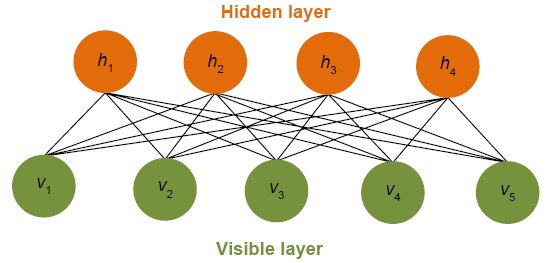
\includegraphics[scale=0.5]{chap4-img/RBM}
	\caption{ماشین بلتزمن محدود}
	\label{chap4-fig1}
\end{figure}

در ترم نهایی در رابطه‌ی
\ref{chap4-eq5}
مشاهده می‌شود که مقدار
$p(\textbf{h}|\textbf{v})$
برابر است با حاصلضرب
$exp$
به ازای تمام ابعاد بردار
$h$,
لذا نتیجه گرفته می‌‌شود که ابعاد بردار
$h$ 
یعنی‌ همان
$h_j$ها
نسبت به یکدیگر دارای استقلال شرطی هستند. در نتیجه می‌توان رابطه‌ی
\ref{chap4-eq5}
را به شکل رابطه‌ی
\begin{align}
	\centering
	\label{chap4-eq6}
	p(\textbf{h}|\textbf{v})=\prod_{j=1}^{H}p(h_j|\textbf{v})	
\end{align}
بازنویسی کرد. همچنین داریم:
\begin{align}
	\centering
	\label{chap4-eq7}
	p(h_j = 1|\textbf{v})=\dfrac{p(h_j=1,\textbf{v})}{p(h_j=1,\textbf{v})+ p(h_j=0,\textbf{v})}
						 &=\dfrac{exp\{\textbf{v}W_j + b_j\}}{exp\{0\} + exp\{\textbf{v}W_j + b_j\}}\\\nonumber
						 &=sigmoid(\textbf{v}W_j + b_j)
\end{align}
\begin{align}
	\centering
	\label{chap4-eq8}
	p(\textbf{h}|\textbf{v})=\prod_{j=1}^{H}sigmoid(\textbf{v}W_j + b_j)
\end{align}
به همین شکل می‌‌توان نتیجه گرفت:
\begin{align}
	\centering
	\label{chap4-eq9}
	p(\textbf{v}|\textbf{h})=\prod_{i=1}^{D}sigmoid(W_i\textbf{h} + a_i)
\end{align}

برای آموزش این مدل فرض می‌‌شود یک مجموعه داده‌ی باینری به صورت
$\{\textbf{v}^{t}\}_{t=1}^{n}$
به عنوان داده‌های آموزش در اختیار است. هدف پیدا کردن پارامتر‌های
$W, \textbf{a}, \textbf{b}$
به صورتی‌ است که لگاریتم درست‌نمایی برای مشاهده‌ی داده‌های آموزش بیشینه باشد. به بیان ریاضی‌ می‌‌خواهیم مقدار رابطه‌ی
\begin{align}
	\centering
	\label{chap4-eq10}
	\ell(W, \textbf{a}, \textbf{b}) &= \sum_{t=1}^{n}\log p(\textbf{v}^t) = \sum_{t=1}^{n}\log \sum_h p(\textbf{v}^t, h)\\\nonumber
	&= \sum_{t=1}^{n}\log\dfrac{1}{Z} \sum_h e^{-E(\textbf{v}^t,h)} = \sum_{t=1}^{n}\log \sum_h e^{-E(\textbf{v}^t,h)} - n\log Z\\\nonumber
	&= \sum_{t=1}^{n}\log\sum_h e^{-E(\textbf{v}^t,h)} - n\log\sum_{\textbf{v},\textbf{h}}exp\left\lbrace -E(\textbf{v}^t,h)\right\rbrace\\\nonumber
\end{align}
را نسبت به مجموعه پارامتر‌های
$\theta = \{W, \textbf{a}, \textbf{b}\}$
بیشینه کنیم.

رابطه‌ی
\ref{chap4-eq10}
را معاد‌له‌ی لگاریتم درست‌نمایی تعریف می‌‌کنیم که برای بیشینه کردن آن نسبت به مجموعه پارامتر‌های
$\theta$
باید از آن نسبت به پارامترهای این مجموعه مشتق گرفت.
\begin{align}
	\centering
	\label{chap4-eq11}
	\triangledown_\theta \ell(\theta) &= \triangledown_\theta \sum_{t=1}^{n} \log \sum_h exp \left\lbrace -E(\textbf{v}^t, \textbf{h}) \right\rbrace - n\triangledown_\theta \log \sum_{\textbf{v}, \textbf{h}} exp \left\lbrace -E(\textbf{v}, \textbf{h}) \right\rbrace \\\nonumber
	&=\sum_{t=1}^{n} \dfrac{\sum_h exp \left\lbrace -E(\textbf{v}^t, \textbf{h}) \right\rbrace \triangledown_\theta -E(\textbf{v}^t, \textbf{h})}{\sum_h exp \left\lbrace -E(\textbf{v}^t, \textbf{h}) \right\rbrace} - n \dfrac{\sum_{v,h} exp \left\lbrace -E(\textbf{v}, \textbf{h}) \right\rbrace \triangledown_\theta -E(\textbf{v}, \textbf{h})}{\sum_{v,h} exp \left\lbrace -E(\textbf{v}, \textbf{h}) \right\rbrace}\\\nonumber
	&=\sum_{t=1}^{n}E_{p(\textbf{h}|\textbf{v}^t)}[\triangledown_\theta -E(\textbf{v}^t, \textbf{h})] - nE_{p(\textbf{v},\textbf{h})}[\triangledown_\theta -E(\textbf{v}, \textbf{h})]
\end{align}
\begin{align}
	\centering
	\label{chap4-eq12}
	\triangledown_{W} -E(\textbf{v},\textbf{h}) = \textbf{v}^T\textbf{h} \qquad  \triangledown_{\textbf{a}} -E(\textbf{v},\textbf{h}) = \textbf{v} \qquad  \triangledown_{\textbf{b}} -E(\textbf{v},\textbf{h}) = \textbf{h}
\end{align}

ترم اول سمت راست رابطه
\ref{chap4-eq11}
یک مقدار مورد انتظار برای مشتق تابع انرژی نسبت به توزیع شرطی دادهای آموزش،
$p(\textbf{h}|\textbf{v})$،
و ترم دوم آن یک مقدار مورد انتظار برای تابع انرژی نسبت به توزیع مشترک برای تمام حالت های  مدل
$p(\textbf{v},\textbf{h})$
 است. با توجه به رابطه‌ی
\ref{chap4-eq12}
برای بدست آوردن ترم اول در رابطه‌ی
\begin{align}
	\centering
	\label{chap4-eq13}
	\triangledown_W \ell(W, \textbf{a}, \textbf{b})=\sum_{t=1}^{n} \textbf{v}^{t^T} \hat{h}^t - nE_{p(\textbf{v},\textbf{h})}[\textbf{v}^T\textbf{h}]
\end{align}
برای هر بردار
$\textbf{v}$
مقدار
$\textbf{h}$
متناظر با آن را با استفاده از رابطه‌ی
\ref{chap4-eq8}
بدست می‌‌آوریم. از آن‌جا که ترم دوم رابطه‌ی
\ref{chap4-eq11}
به توزیع تمام حالات موجود برای مدل
($p(\textbf{v},\textbf{h})$)
وابسته است محاسبه‌ی آن برای ما امکان‌پذیر نیست و باید مقدار آن را به صورت تقریبی بدست آوریم. الگوریتم
CD
در اینجا وارد عمل می‌شود و مقدار مورد انتظار از مشتق تابع انرژی بر روی یک توزیع مشترک را با یک تخمین نقطه‌ای جایگزین می‌‌کند. به این صورت که یک بردار از داده‌های آموزش انتخاب کرده و با استفاده از الگوریتم نمونه‌برداری
Gibbs
و همچنین روابط
\ref{chap4-eq9}
و
\ref{chap4-eq8}
مقادیر بردار‌های
$\textbf{h}$
و
$\textbf{v}$
را به ترتیب محاسبه می‌کند. یک چرخه‌‌ی کامل الگوریتم نمونه‌برداری
Gibbs
شامل محاسبه‌ی بردار
$\textbf{h}$
از یک بردار
$\textbf{v}$
و سپس ساختن مجدد بردار
$\textbf{v}$
از این بردار
$\textbf{h}$
است. این چرخه تا زمانی که به یک حالت تعادل دست یابید ادامه پیدا می‌کند، در حالت تعادل مقدار بردارهای
$\textbf{v}$
و
$\textbf{h}$
بدست آماده برابر با مقدار مورد انتظار برای ترم دوم رابطه
\ref{chap4-eq13}
در نظر گرفته می‌‌شود. همچنین با استفاده از مقادیر بدست آمده برای بردارهای
$\textbf{v}$
و
$\textbf{h}$
مقدار روابط
\begin{align}
	\centering
	\label{chap4-eq14}
	\triangledown_{\textbf{a}} \ell(W, \textbf{a}, \textbf{b})=\sum_{t=1}^{n} \textbf{v}^{t} - nE_{p(\textbf{v},\textbf{h})}[\textbf{v}] 
\end{align}
و
\begin{align}
	\centering
	\label{chap4-eq15}
	\triangledown_{\textbf{b}} \ell(W, \textbf{a}, \textbf{b})=\sum_{t=1}^{n} \textbf{h}^{t} - nE_{p(\textbf{v},\textbf{h})}[\textbf{h}] 
\end{align}
نیز محاسبه می‌‌گردد.

همان‌طور که پیش از این در بخش
\ref{chap2sec7}
بیان شد، آقای
Hinton
نشان داد که تنها تعداد کمی‌ چرخه‌‌‌ی نمونه‌برداری
Gibbs
برای بدست آوردن تقریبی مناسب نسبت به توزیع
$p(\textbf{v},\textbf{h})$
کافی‌ است
\cite{hinton2002training}\cite{carreira2005contrastive}.
اگرچه پیاده‌سازی‌های انجام شده نشان داده است که تنها انجام یک چرخه‌ی
Gibbs
برای محاسبه‌ی یک تقریب صحیح از جهت حرکت گرادیان کافی‌ است
\cite{carreira2005contrastive}.
در نهایت برای کمینه کردن تابع انرژی رابطه‌ی بروز‌رسانی کردن مجموعه پارامتر‌های 
$\theta$
 به شکل رابطه‌ی
\begin{align}
	\centering
	\label{chap4-eq16}
	\theta_{t+1} = \theta_t + \epsilon \left( E_{P_{data}}[\triangledown_{\theta} -E(\textbf{v},\textbf{h})] - E_{P_{model}}[\triangledown_{\theta} -E(\textbf{v},\textbf{h})] \right) 
\end{align}
می‌گردد که در آن
$\epsilon$
ضریب یادگیری است و به صورت تجربی‌ مشخص گردد.


\section{ماشین بلتزمن محدود با واحدهای قابل مشاهده صحیح}
\label{chap4sec3}
ساختار معرفی‌ شده در بخش
\ref{chap4sec2}
مدل استاندارد
RBM
است که به صورت دقیق مورد بررسی‌ قرار گرفت و به عنوان مدل پایه برای روش پیشنهادی در این پایان‌‌نامه در نظر گرفته می‌‌شود. برای تعریف ساختار مورد نظر در این پایان‌‌نامه جهت مدل‌سازی احساس و موضوع نیاز به معرفی‌ و بررسی‌ نمونه‌های پیچیده‌تری از مدل
RBM
استاندارد است.

محدود بودن به حالت باینری برای داده‌های ورودی و همچنین طول ثابت برای آن‌ها دو اشکال اساسی در مدل
RBM
استاندارد هستند. حال فرض کنید ساختاری داریم که در آن داده‌های ورودی همچنان دارای طول ثابت هستند اما به جای حالت باینری می‌‌توانند هر مقدار صحیح غیر منفی‌ از یک حداقل تا یک حداکثر را اختیار کنند. در این ساختار که در شکل
\ref{chap4-fig2}
نشان داده شده است به جای بردار ورودی ما ماتریس ورودی خواهیم داشت، و هر داده به صورت یک ماتریس با درایه‌های ۰ و ۱ به مدل وارد می‌‌شود. در مدل
RBM
استاندارد ورودی تنها یک بردار با طول ثابت با درایه‌های ۰ و یا ۱ بود، که حضور و یا عدم حضور هر یک از ویژگی‌‌های متناظر با درایه‌ی مورد نظر در بردار ورودی را مشخص می‌‌کند. اما در این مدل هر داده‌ی ورودی به صورت ماتریسی متشکل از ۰ یا ۱ است.

فرض کنید در مساله‌ای‌ که با آن سرو کار داریم هر داده‌ی ورودی دارای
D
ویژگی‌ است که هر یک از این ویژگی‌ها می‌‌توانند 
K
مقدار داشته باشند. مدل
RBM
استاندارد توانایی کار کردن با یک چنین داده‌های ورودی را ندارد چرا که در آن داده‌های ورودی تنها می‌‌توانند یک بردار با طول ثابت و شامل ۰ و ۱ باشند. در این مدل جدید هر داده‌ی ورودی به صورت ماتریسی با اندازه
$K \times D$
در نظر گرفته می‌شود که همان‌طور که بیان شد
D
طول بردار ورودی یا همان تعداد ویژگی‌های مساله و
K
بیشینه مقداری است که هر ویژگی‌ می‌‌تواند داشته باشد. برای ساخت این ماتریس ابتدا تمام درایه‌های آن را صفر می‌‌کنیم و سپس برای هر ستون یا به عبارتی برای هر ویژگی‌ سطر متناظر با مقدار آن ویژگی‌ را ۱ می‌‌کنیم. در این حالت به ازای هر داده‌ی ورودی یک ماتریس شامل ۰ و ۱ داریم با این خصوصیت که در هر ستون آن تنها مقدار یک سطر  ۱ است و مابقی سطرها مقدارشان ۰ است.
\begin{figure}[!t]
	\centering
	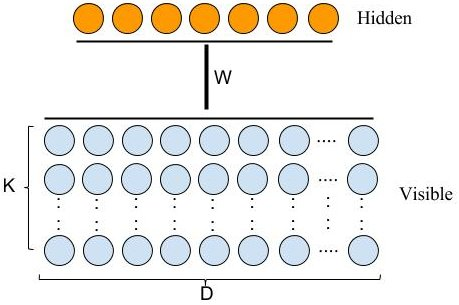
\includegraphics[scale=0.5]{chap4-img/MRBM}
	\caption{ماشین بلتزمن محدود با واحدهای قابل مشاهده صحیح}
	\label{chap4-fig2}
\end{figure}

تا به اینجا تفاوت این ساختار با مدل
RBM
استاندارد را معرفی‌ کردیم. از نظر تفاوت در فضای پارامتری، در مدل
RBM
استاندارد ماتریس وزن بین لایه‌ی قابل مشاهده و لایه‌ی پنهان یک ماتریس دو بعدی بود، اما در این ساختار به دلیل تغییر در شکل ورودی ماتریس وزن بین این دو لایه یک ماتریس سه بعدی است. در این ساختار نیز مانند مدل
RBM
استاندارد که در آن تمام ابعاد بردار ورودی به تمام واحد‌های لایه‌ی پنهان متصل بودند، در اینجا نیز یک اتصال کامل بین تمام قسمت‌های ماتریس ورودی و تمام واحد‌های لایه‌ی پنهان بر قرار است. تفاوت دیگر این دو ساختار در فضای پارامتر‌ها مربوط به بایاس لایه‌ی قابل مشاهده است. برخلاف مدل
RBM
استاندارد که برای لایه‌ی قابل مشاهده یک بردار بایاس وجود داشت در ساختار نشان داده شده در شکل
\ref{chap4-fig2}
ما یک ماتریس دو بعدی برای بایاس خواهیم داشت که در فرآیند آموزش درایه‌های آن یاد گرفته می‌‌شوند.

با توجه به تغییرات بیان شده در ساختار
RBM
استاندارد و همچنین تغییرات اعمال شده در فضای پارامتر‌های مساله، روابط
\ref{chap4-eq1}
تا
\ref{chap4-eq9}
نیز دچار تغییرات اساسی‌ می‌‌گردند که در اینجا به بیان آن‌ها می‌پردازیم. فرض کنید قصد مدل‌سازی بردا‌های ورودی
$\textbf{v}$
با مدلی‌ مانند آنچه در شکل
\ref{chap4-fig2}
نشان داده شده است را داریم. اگر هر داده‌ی
$\textbf{v}$
به شکل
$\textbf{v} \in \{1, ..., K\}^D$
باشد، که در آن همان‌طور که پیش از این بیان کردیم،
$K$
بیشینه مقداری است که هر ویژگی‌ می‌‌تواند دریافت کند و
$D$
اندازه داده‌های ورودی است. همچنین بردار پنهان به شکل
$\textbf{h} \in \{0,1\}^H$
می‌ باشد. اگر
$\textbf{V}$
ماتریس باینری قابل مشاهده باشد که برای هر داده‌ی ورودی ساخته می‌‌شود، در این صورت تابع انرژی برای حالت
$\{\textbf{V},\textbf{h}\}$
به شکل
\begin{align}
	\centering
	\label{chap4-eq17}
	E(\textbf{V},\textbf{h})=-\sum_{i=1}^{D}\sum_{j=1}^{H}\sum_{k=1}^{K}W_{ijk}h_jv_{ik}-\sum_{i=1}^{D}\sum_{k=1}^{K}v_{ik}a_{ik} - \sum_{j=1}^{H}h_jb_j
\end{align}
تعریف می‌‌شود.

در رابطه‌ی‌
\ref{chap4-eq17}
نیز مانند حالت قبل
$\{W, a, \textbf{b}\}$
مجموعه پارامتر‌های مدل هستند که در آن
$W_{D \times H \times K}$
ماتریس سه‌ بعدی وزن بین واحد قابل مشاهده‌ی
$i$ام
 و مقدار
$k$ام
 و واحد
$j$ام 
بردار لایه‌ی پنهان است، همچنین در رابطه‌ی
\ref{chap4-eq17}، $a_{D \times K}$
ماتریس دو بعدی بایاس برای لایه‌ی قابل مشاهده و
$\textbf{b}_{1 \times H}$
بردار بایاس برای لایه‌ی پنهان است. احتمالی‌ که این ساختار به ماتریس باینری قابل مشاهده‌ی
$\textbf{V}$
اختصاص می‌‌دهد از
 \begin{align}
 	\centering
 	\label{chap4-eq18}
 	p(\textbf{V}) = \sum_{h} \dfrac{1}{Z} e^{-E(\textbf{V},\textbf{h})} \quad\quad ; \quad
 	Z = \sum_{\textbf{V},\textbf{h}} e^{-E(\textbf{V},\textbf{h})} 
 \end{align}
 بدست می‌‌آید.


در این ساختار توزیع‌های شرطی برای لایه‌های قابل مشاهده و پنهان به شکل
\begin{align}
	\centering
	\label{chap4-eq19}
	p(v_{ik}=1|\textbf{h})=\dfrac{exp(a_{ik}+\sum_{j=1}^{H}h_jW_{ijk})}{\sum_{k=1}^{K}exp(a_{ik}+\sum_{j=1}^{H}h_jW_{ijk})}
\end{align}
و
\begin{align}
	\centering
	\label{chap4-eq20}
	p(h_{j}=1|\textbf{V})=\sigma \left( b_j +  \sum_{i=1}^{D}\sum_{k=1}^{K}W_{ijk}v_{ik} \right)
\end{align}
هستند. همان‌طور که مشاهده می‌‌گردد توزیع شرطی مربوط به لایه‌ی قابل مشاهده کاملا با رابطه‌ی
\ref{chap4-eq9}
که برای مدل
RBM
استاندارد تعریف گردید تفاوت دارد، و توزیع مورد استفاده در رابطه‌ی
\ref{chap4-eq19}
 مانند آنچه که در بخش
\ref{chap2sec9}
توضیح داده شد از تابع
Softmax
استفاده می‌‌کند. دلیل استفاده از تابع
Softmax
به جای تابع سیگموید که در مدل
RBM
استاندارد از آن استفاده می‌‌شد تغییر در ساختار ورودی و لایه‌ی قابل مشاهده است. با توجه به اینکه هر ویژگی‌ تنها یک مقدار از
$K$
مقدار ممکن را می‌‌تواند داشته باشد، یا به عبارتی در هر ستون ماتریس باینری
$\textbf{V}$
 در لایه‌ی قابل مشاهده تنها یک ۱ می‌‌تواند وجود داشته باشد، لذا برای هر ستون در این ماتریس از یک تابع
Softmax
استفاده می‌گردد و احتمال یک بودن هر یک از این
$K$
 مقدار حساب می‌گردد و سپس با تولید یک عدد تصادفی با توجه به احتمالات بدست آمده برای هر یک از
$K$
مقدار ممکن برای هر ویژگی‌، مقدار آن ویژگی‌ تعیین می‌‌گردد. در حقیقت فرمول
\ref{chap4-eq19}
برای توزیع احتمالی‌ لایه قابل مشاهده این اطمینان را به ما می‌دهد که مقادیر بدست آماده برای هر ویژگی‌ به ازای
$K$
مقدار ممکن برای آن، یک توزیع چند احتمالی‌ چندجمله‌ای ازدرجه‌ی
$K$
است.



\section{مدل مولد براساس تعداد کلمات}
\label{chap4sec4}

مدلی‌ که در این بخش به صورت کامل آن را شرح می‌‌دهیم و گسترش یافته‌ی مدل معرفی‌ شده در بخش
\ref{chap4sec3}
است در واقع همان مدل
RS
 است که در بخش
\ref{chap3sec3sub5}
به صورت مختصر آن را معرفی‌ کردیم. بررسی‌ مدل
RS
در درک مدل پیشنهادی حائز اهمیت است، چرا که مدل پیشنهادی در این پایان‌‌نامه بر روی ساختار این مدل سوار شده و گسترش یافته‌ی آن است. مدل
RS
 همان‌طور که در بخش
\ref{chap3sec3sub5}
بیان شد یک مدل مولد احتمالی‌ بر اساس تعداد کلمات است که به صورت بدون نظارت به مدل‌سازی موضوع در داده‌های متنی می‌‌پردازد.

در بحث مدل‌سازی موضوع پیش از آموزش مدل ابتدا یک بار تمام مجموعه سند پیمایش می‌‌شود و تمام کلمات متمایز در تمام اسناد مشخص شده و همراه با ایندکس هرکدام ذخیره می‌‌شوند. به عبارت دیگر قبل از شروع مرحله‌ی آموزش ابتدا یک لغت‌نامه از تمام کلمات متمایز در مجموعه اسناد ساخته می‌‌شود. پس از پایان این مرحله و ساخت لغت‌نامه به مدل بخش
\ref{chap4sec3}
بر می‌‌گردیم و مدل معرفی‌ شده در آن جا را در این حالت اندکی‌ بررسی‌ می‌‌کنیم. در بخش
\ref{chap4sec3}
گفته شد که مقدار هر ویژگی‌ می‌‌تواند از یک کمینه تا یک بیشینه باشد، حال فرض کنید که بحث مدل‌سازی موضوع بر روی داده‌های متنی است و پس از ساخت لغت‌نامه می‌خواهیم از مدل بخش
\ref{chap4sec3}
استفاده کنیم. در اینجا مقدار هر ویژگی‌ برابر با اندیس یکی‌ از کلمات لغت‌نامه است. هر سند ورودی پس از انجام پیش پردازش‌های لازم به صورت یک دنباله از کلمات تبدیل شده است که هر کدام از این کلمات برابر با یکی‌ از کلمات لغت‌نامه هستند. به این ترتیب در ماتریس ورودی به مدل که یک ماتریس به انداز‌ه‌ی
$K \times D$
می‌ باشد
$K$
برابر با اندازه لغت‌نامه است و
$D$
نشان دهنده‌ی طول سند متنی است. در این حالت برای هر ستون مقدار سطر متناظر با اندیس آن کلمه در لغت‌نامه برابر با ۱ می‌‌شود و دیگر درایه‌های آن ستون همچنان صفر باقی‌ می‌‌مانند.

حال فرض کنید که برای مدل کردن داده‌های متنی با استفاده از ساختار معرفی‌ شده در بخش
\ref{chap4sec3}
برای هر سند یک شبکه‌ی
RBM
جدا می‌‌سازیم که به تعداد کلمات همان سند دارای واحد
Softmax
است. در این حالت ورودی دیگر یک ماتریس باینری نخواهد بود و به صورت برداری از تعداد کلمات موجود در آن سند است که می‌‌توانیم ترتیب را در آن‌ها نادیده بگیریم. رابطه‌ی محاسبه‌ی انرژی در این حالت به شکل
\begin{align}
	\centering
	\label{chap4-eq21}
	E(\textbf{v},\textbf{h})=-\sum_{j=1}^{H}\sum_{k=1}^{K}W_{jk}h_j\hat{v}_{k}-\sum_{k=1}^{K}v_{k}a_{k} - D\sum_{j=1}^{H}h_jb_j
	\end{align}
است که در آن
$\hat{v}^k = \sum_{i=1}^{D}v_{ik}$
است. به عبارت دیگر
$\hat{\textbf{v}}$
برداری است با طول
$K$
که 
$K$
همان اندازه لغت‌نامه است و از محاسبه‌ی حاصل جمع سطر‌های ماتریس باینری ورودی بدست می‌‌آید.
با تغییرات انجام گرفته در لایه‌ی قابل مشاهده و تعویض ساختار ورودی، در ماتریس وزن بین این لایه و لایه‌ی پنهان و همچنین بایاس لایه‌ی قابل مشاهده تغییراتی‌ رخ می‌‌دهد. در رابطه
\ref{chap4-eq21}، $W$
ماتریسی با اندازه‌ی
$K \times H$
و
$\textbf{a}$
یک بردار با اندازه‌ی
$1 \times K$
هستند.

در این مدل که آن را
Softmax
تکرار شده نامیدیم روابط شرطی محاسبه‌ی لایه‌ی قابل مشاهده و لایه‌ی پنهان به شکل
\begin{align}
	\centering
	\label{chap4-eq22}
	p(v_{i}=w|\textbf{h})=\dfrac{exp(a_{w}+\sum_{j=1}^{H}h_jW_{wj})}{\sum_{k=1}^{K}exp(a_{w}+\sum_{j=1}^{H}W_{wj})}
	\end{align}
و
\begin{align}
	\centering
	\label{chap4-eq23}
	p(h_{j}=1|\textbf{V})=\sigma \left( Db_j + \sum_{k=1}^{K}W_{kj}\hat{v}_k \right)
\end{align}
هستند.

همان‌طور که مشاهده می‌‌شود در روابط
\ref{chap4-eq21}
و
\ref{chap4-eq23}
ترم بایاس برای لایه‌ی پنهان با اندازه سند جاری نیز متناسب است. وجود این تناسب در پیاده‌سازی‌های تجربی‌ و هنگامی که با اسناد با طول‌های متفاوت سر و کار داریم بسیار حیاتی است. در این مدل نیز برای آموزش از الگوریتم
CD
استفاده می‌‌شود، رابطه‌ی به روزرسانی نیز همان است که در بخش
\ref{chap4sec2}
و رابطه
\ref{chap4-eq16}
نشان داده شد با این تفاوت که به جای بردار باینری برای لایه‌ی قابل مشاهده از مقدار آن بر اساس تعداد کلمات استفاده می‌‌شود. برای مثال در یک مجموعه از
N
سند آموزش که به شکل
$\{\textbf{V}_n\}_{n=1}^{N}$
است رابطه‌ي به روزرسانی برای یک عنصر ماتریس وزن به شکل
\begin{align}
	\centering
	\label{chap4-eq24}
	\dfrac{1}{N}\sum_{n=1}^{N}\dfrac{\partial\log P(\textbf{V}_n)}{\partial W_{jk}} = E_{P_{data}}[\hat{v}_kh_j]-E_{P_{model}}[\hat{v}_kh_j]
\end{align}
\begin{align}
	\centering
	\label{chap4-eq25}
	\triangle W_{jk} = \alpha \left( E_{P_{data}}[\hat{v}_kh_j]-E_{P_{model}}[\hat{v}_kh_j]  \right)
\end{align}
است.


\section{مدل پیشنهادی مولد احتمالی احساس/موضوع}
\label{chap4sec5}



مدل معرفی‌ شده در این پایان‌‌نامه یک مدل مولد احتمالاتی شبکه عصبی برای مدل‌سازی موضوع و احساس در داده‌های متنی است. این روش گسترش یافته‌ی مدل
RS
است که در بخش
\ref{chap4sec4}
معرفی شد. در مدل پیشنهادی که در شکل
\ref{chap4-fig3}
نشان داده شده است، مشاهده می‌‌گردد که این روش نیز یک ساختار دو لایه دارد که در سمت لایه‌ی قابل مشاهده‌ی آن یک بردار متناظر با برچسب هر سند که در این پایان‌‌نامه ما آن را به عنوان بردار متناظر با احساس هر سند تعبیر می‌کنیم به ساختار مدل اضافه شده است. بردار ورودی در این ساختار در قسمت
Visible
یک بردار با طولی ثابت و به اندازه‌ی اندازه لغت‌نامه یا همان تعداد کلمات متمایز در متن است که در آن تعداد تکرار کلمات مشخص شده است.

در مدل معرفی‌ شده در بخش
\ref{chap4sec3}
که در شکل
\ref{chap4-fig2}
نشان داده شده است، هر سند ورودی پس از انجام پیش‌پردازش‌های مورد نیاز و تبدیل به یک دنباله از کلمات به صورت یک ماتریس به مدل وارد می‌‌شود. در نظر گرفتن یک چنین ساختاری برای هر سند ورودی به این معنی‌ است که جایگاه هر کلمه در متن برای ما مهم است و ترتیب کلمات در هر سند درنظر گرفته می‌‌شود که این امر موجب بزرگ شدن فضای پارامتر‌های مساله (سه‌ بعدی شدن ماتریس وزن و دو بعدی شدن ماتریس بایاس برای لایه‌ی قابل مشاهده) و کند شدن فرآیند آموزش می‌‌گردد. علاوه بر این در بحث مدل‌سازی موضوع حضور و عدم حضور کلمات به همراه فرکانس تکرار آن‌ها دارای اهمیت است نه محل قرار گرفتن هر کلمه در متن، چرا که تمام مدل‌های بررسی‌ شده در این پایان‌‌نامه و همچنین مدل پیشنهادی بر اساس کیسه کلمات
(\ref{chap2sec10})
رفتار می‌‌کنند که در آن ترتیب کلمات در نظر گرفته نمی‌‌شود.  در شکل
\ref{chap4-fig4}
یک نمونه از ماتریس ورودی به مدل معرفی‌ شده در بخش
\ref{chap4sec3}
نشان داده شده است. در این مثال سند ورودی به مدل پس از انجام پیش‌پردازش‌های لازم به یک دنباله از پنج کلمه تبدیل شده است، یک کلمه از لغت‌نامه  مانند 
Student
در سند ورودی در دو جایگاه مختلف در سند نشان داده شده است، با توجه به ساختار معرفی‌ شده در بخش
\ref{chap4sec3}
و ماتریس‌های وزن و بایاس سه‌ و دو بعدی، نتیجه گرفته می‌‌شود برای این کلمه دو مقدار متفاوت برای وزن و بایاس آن (یکی برای x
 و یکی برای 
 (y
 تعریف می‌‌شود. لذا متناسب با اینکه کلمه در کجای سند ورودی قرار داشته باشد می‌تواند وزن‌های متفاوتی داشته باشد. این امر موجب بزرگ شدن ماتریس ورودی،  طولانی‌ شدن فرایند آموزش و در نظر گرفتن تفاوت برای محل قرار گرفتن هر کلمه در متن می‌گردد. در مدل پیشنهادی در این پایان‌‌نامه که در ادامه شرح داده می‌‌شود با تغییر ساختار ورودی از این مشکلات اجتناب می‌‌گردد.

\begin{figure}[!t]
	\centering
	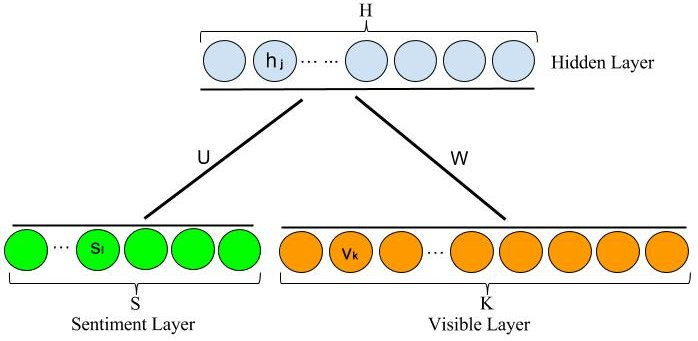
\includegraphics[scale=0.5]{chap4-img/SRS}
	\caption{مدل پیشنهادی مولد احتمالی احساس/موضوع با Softmax تکرار شده}
	\label{chap4-fig3}
\end{figure}

\begin{figure}[!t]
	\centering
	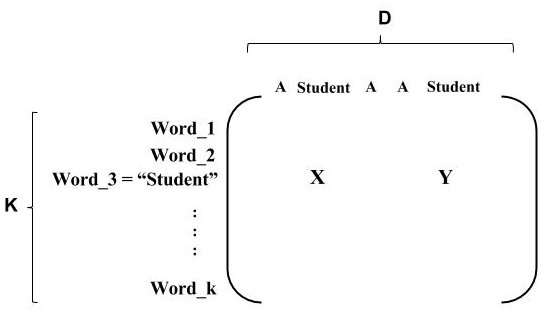
\includegraphics[scale=0.4]{chap4-img/example}
	\caption{یک سند ورودی با ۵ کلمه در مدل بخش \ref{chap4sec3}}
	\label{chap4-fig4}
\end{figure}

در مدل پیشنهادی در این پایان‌‌نامه و همچنین مدل
RS
هر سند به صورت یک بردار شامل تعداد کلمات به مدل وارد می‌‌شود. در این ساختار مانند آنچه که در شکل
\ref{chap4-fig3}
نشان داده شده است طول بردار ورودی برابر با اندازه لغت‌نامه یا همان تعداد کلمات متمایز در مجموعه سند در نظر گرفته می‌‌شود که درایه‌های آن تعداد تکرار هر کلمه از لغت‌نامه در سند جاری را نشان می‌‌دهند. در این حالت در واقع وزن‌ها برای هر کلمه به اشتراک گذاشته می‌‌شوند فارغ از اینکه این کلمه در کجای سند ورودی قرار دارد. به طور مثال برای کلمه‌ی‌
$n$ام 
لغت‌نامه یک وزن و یک بایاس تعریف می‌‌گردد و این کلمه در هر جای سند ورودی قرار داشته باشد وزنش تغییری نخواهد کرد و در فرآیند آموزش تنها یک وزن و یک بایاس برای هر کلمه یاد گرفته می‌‌شود. با توجه به ساختار مدل که در شکل
\ref{chap4-fig3}
نشان داده شده است، برای هر سند متنی برداری با اندازه لغت‌نامه که شامل تعداد تکرار هر کلمه از لغت‌نامه در آن سند است و همچنین یک بردار باینری که نشان دهنده احساس سند جاری است به عنوان ورودی به شبکه وارد می‌‌شوند، و توزیع‌های موجود برروی کلمات مختلف در هر موضوع و همچنین احساس مرتبط با آن‌ها توسط مدل در لایه‌‌ی پنهان استخراج می‌‌شوند.

مدل پیشنهادی در این پایان‌‌نامه 
(شکل \ref{chap4-fig3})
 یک مدل نظارت شده است که برای هر سند با کمینه کردن یک تابع انرژی که به شکل
\begin{align}
	\label{chap4-eq26}
	E(\textbf{V},\textbf{s},\textbf{h})=-\sum_{j=1}^{H}\sum_{k=1}^{K}W_{kj}h_j\hat{v}_{k}&-\sum_{j=1}^{H}\sum_{l=1}^{S}U_{lj}h_js_l\\\nonumber
	&-\sum_{k=1}^{K}v_{k}a_{k} -\sum_{l=1}^{S}s_lc_l- D\sum_{j=1}^{H}h_jb_j
\end{align}
تعریف می‌‌شود، به مدل‌سازی احساس و موضوع به صورت مشترک در داده‌های متنی می‌‌پردازد. با اضافه شدن یک لایه‌ی جدید در این مدل به همراه ماتریس وزن و همچنین بردار بایاس همراه با آن، روابط موجود نسبت به ساختار‌های پیشین تغییر می‌کند. همان‌طور که در رابطه‌ی
\ref{chap4-eq26}
مشاهده می‌‌شود، برای محاسبه‌ی انرژی در مدل پیشنهادی ترم‌های مربوط به وزن و بایاس لایه‌ی احساس نیز در بدست آوردن مقدار نهایی مشارکت دارند. پس از محاسبه‌ی مقدار انرژی به کمک رابطه‌ی
\ref{chap4-eq26}،
 با استفاده از
\begin{align}
	\centering
	\label{chap4-eq27}
	p(\textbf{v},\textbf{s},\textbf{h}) = \dfrac{1}{Z} e^{-E(\textbf{v},\textbf{s},\textbf{h})} \Rightarrow
	p(\textbf{v},\textbf{s}) = \dfrac{1}{Z} \sum_{h}  e^{-E(\textbf{v},\textbf{s},\textbf{h})} \ \ ,
	Z = \sum_{\textbf{v}}\sum_{\textbf{s}}\sum_{\textbf{h}} e^{-E(\textbf{v},\textbf{s},\textbf{h})} 
\end{align}
احتمالی‌ که مدل به هر سند و ‌لایه‌ی احساس همراه با آن اختصاص می‌‌دهد، محاسبه می‌‌گردد. برای آموزش این مدل و بروزرسانی پارامترهای شبکه که شامل ماتریس‌های وزن بین لایه‌ی قابل‌مشاهده و پنهان و همچنین لایه‌ی احساس و پنهان هستند و همچنین بایاس‌های هر سه‌ لایه از الگوریتم
CD
که در بخش
\ref{chap2sec7}
معرفی‌ شده به شکل
\begin{align}
	\centering
	\label{chap4-eq28}
	\triangle\theta = \alpha \left( E_{P_{data}}[\theta]-E_{P_{model}}[\theta]\right) \Rightarrow \theta_{t+1} = \theta_t + \triangle\theta
\end{align}
استفاده می‌‌شود.
در رابطه
\ref{chap4-eq26}، $\theta=\{W, U, \textbf{a}, \textbf{b}, \textbf{c} \}$
مجموعه پارامتر‌های مدل است که در آن
$W_{K \times H}$
ماتریس وزن بین بردار
$Visible$
و لایه‌ی
$Hidden$، $U_{S \times H}$
ماتریس وزن بین لایه‌ی
$Sentiment$
و لایه‌ی
$Hidden$
و
$\textbf{a}$، $\textbf{b}$
و
$\textbf{c}$
به ترتیب بردار‌های بایاس لایه‌ی
$Visible$، $Hidden$
و
$Sentiment$
می‌ باشند. لازم به ذکر است که
$K$
و
$H$
مانند آنچه در بخش‌های پیشین ذکر کردیم به ترتیب اندازه لغت‌نامه و طول لایه‌ی پنهان هستند و
$S$
به عنوان تعداد احساس موجود یا اندازه بردار
$Sentiment$
تعریف می‌‌شود.

در مدل پیشنهادی روابط شرطی برای محاسبه‌ی هر یک از لایه‌های
$Visible$، $Sentiment$
و
$Hidden$
 به شکل
\begin{align}
	\centering
	\label{chap4-eq29}
	p(v_{i}=w|\textbf{h})=\dfrac{exp(a_{w}+\sum_{j=1}^{H}W_{wj}h_j)}{\sum_{k=1}^{K}exp(a_{w}+\sum_{j=1}^{H}W_{wj}h_j)}
\end{align}
\begin{align}
	\centering
	\label{chap4-eq30}
	p(s_{l}=1|\textbf{h})=\dfrac{exp(c_{l}+\sum_{j=1}^{H}U_{lj}h_j)}{\sum_{l=1}^{S}exp(c_{l}+\sum_{j=1}^{H}U_{lj}h_j)}
\end{align}
\begin{align}
	\centering
	\label{chap4-eq31}
	p(h_{j}=1|\textbf{v},\textbf{s})=\sigma \left( Db_j + \sum_{k=1}^{K}W_{kj}\hat{v}_k + \sum_{l=1}^{S}U_{lj}s_l \right)
\end{align}
هستند. در اینجا چون مقدار لایه‌ی
$Hidden$
به هر دو مقدار لایه‌ی
$Visible$
و
$Sentiment$
وابسته است، لذا مشاهده می‌‌شود که در رابطه‌ی
\ref{chap4-eq31}
برای مقدار لایه‌ی
$Hidden$
از یک توزیع شرطی که وابسته به هر دو مقدار لایه‌های
$Visible$
و
$Sentiment$
است نمونه گرفته می‌‌شود. اما با توجه به اینکه با داشتن مقدار لایه‌ی
$Hidden$
بردارهای
$Visible$
و
$Sentiment$
از یکدیگر مستقل شرطی هستند لذا در روابط
\ref{chap4-eq29}
و
\ref{chap4-eq30}
مقدار این دو بردار از یک توزیع شرطی که تنها به مقدار بردار
$Hidden$
وابسته است نمونه گرفته می‌‌شوند.

با توجه به خصوصیات بیان شده برای تابع
$Softmax$
در بخش
\ref{chap2sec9}
و توجه به این امر که خروجی برای این تابع متناظر با مقادیر یک توزیع احتمالی‌ چندجمله‌ای است، لذا همان‌طور که مشاهده می‌‌شود، در روابط
\ref{chap4-eq29}
و
\ref{chap4-eq30}
برای محاسبه‌ی مقادیر لایه‌های
$Visible$
و
$Sentiment$
از یک تابع
$Softmax$
استفاده می‌‌گردد. در فرآیند آموزش با استفاده از الگوریتم
CD
برای بدست آوردن مقدار بازسازی\footnote{Reconstruct}
 شده از لایه‌ی
$Visible$
مشروط به بردار
$Hidden$
از رابطه‌ی
\ref{chap4-eq29}
که به صورت
$Softmax$
است، استفاده می‌‌شود. در واقع دلیل اینکه این رابطه و رابطه‌ی
\ref{chap4-eq30}
برای لایه‌ی
$Sentiment$
به فرم تابع
$Softmax$
هستند همین امر است، که پس از محاسبه‌ی مقادیر این لایه‌ها مشروط به بردار
$Hidden$
نیاز به تولید نمونه و نمونه‌برداری از این مقادیر بدست آمده داریم. در نتیجه استفاده از تابع
$Softmax$
برای ما تضمین می‌‌کند که مقادیر محاسبه شده برای این دو بردار یک توزیع احتمالی‌ چندجمله‌ای خواهد بود که می‌‌توان به راحتی‌ از آن نمونه تولید کرد.



%
%رابطه‌ی دیگری که در اینجا از آن برای تشخیص احساس یک سند استفاده می‌‌کنیم و در بحث طبقه‌بندی احساس برای یک سند از پیش دیده نشده کاربرد فراوان دارد به شکل رابطه‌ی
%\ref{chap4-eq32}
%می‌ باشد
%\cite{salakhutdinov2007restricted}.
%\begin{align}
%	\centering
%	\label{chap4-eq32}
%	p(s_l|\textbf{v})=\dfrac{e^{s_l}\prod_{j=1}^{H}\left( 1+ e^{b_j +U_{lj} +\sum_k W_{kj}\hat{v}_k}\right)}{\sum_le^{s_l}\prod_{j=1}^{H}\left( 1+ e^{b_j +U_{lj} +\sum_k W_{kj}\hat{v}_k}\right)}
%\end{align}

\section{نتیجه‌گیری}
در این بخش کلیت نظری مدل پیشنهادی توضیح داده شد. در ابتدا مدل
RBM
به عنوان ساختار پایه برای مدل پیشنهادی در این پایان‌‌نامه مطرح و به صورت کامل بررسی‌ گردید. پس از آن دو روش گسترش یافته از مدل
RBM
که مدل پیشنهادی در این پایان‌‌نامه تعمیم یافته‌ی ‌آن‌ها برای مدل‌سازی احساس و موضوع است به صورت دقیق مورد بررسی‌ قرار گرفتند. سپس مدل پیشنهادی در این پایان‌‌نامه به همراه روابط ریاضی‌ و مؤلفه‌های موجود در آن به صورت کامل توضیح و اثبات گردیدند.

در فصل بعدی جزییات بیشتری در مورد شبیه‌سازی مدل‌ پیشنهادی و نتایج حاصل شده از آن تشریح می‌شود.






